A \emph{Transaction Processing System (TPS)} runs atop an underlying 
key-value store and allows users to bundle multiple data operations 
into a single atomic transaction. Section~\ref{ssec:data-model} describes the NoSQL data 
model and the data access API, and  Section~\ref{ssec:transactions} defines transaction semantics
provided by the TPS. Section~\ref{ssec:schema} provides  background on the modus operandi 
of existing TPSs that support SI,  including Omid. Finally, Section~\ref{ssec:bigdata} zooms 
in on the specifics of HBase and Phoenix. 

\subsection{Data store API}
\label{ssec:data-model}

The  data store holds  \emph{objects} (often referred to as \emph{rows} or {\em records}) identified by unique \emph{keys}.
Each row can consist of multiple \emph{fields}, representing different \emph{columns}. 
We consider multi-versioned objects, where object values are associated with \emph{version numbers}, and
multiple versions associated with the same key may co-exist.
\remove{
Thus, at any given time, an object holds a tuple \tuple{key,\tuple{version,value}+}, where value
can be structured to consist of multiple columns.
}
We further assume that a write operation can specify the version number it writes to.
%monotonically increasing ??
%\paragraph{API} 
The  data store provides the following API:
\begin{description}
\item [\code{get(key, version)}] --  returns the requested version of key.
%if no version is provided, returns the latest; 
%if no field is provided returns the entire record. 
%\item 
The API further allows traversing (reading) earlier versions of the same key.
% in descending order.
\item [\code{update(key, version, fields, values)}] -- 
creates or updates an object, setting the specified fields to the specified values. 
If the version already exists, its value is updated; otherwise, a new version is added. 
\remove{The data store may buffer the write in memory until an ensuing flush. }
\item [\code{remove(key, version)}] -- removes an object with the given key and version.
\item [\code{check\&mutate(key, version, field, old, new)}] -- checks the record associated with key and version. 
If field holds old, replace it with new   and return true; otherwise return false.
\remove{ \item [\code{flush}] -- persists all previous updates to disk.}
%data stores often provide means to atomically read and update a single object, e.g., HBase exports check\&mutate operations, which are 
%internally implemented using a per-row RW lock.
%, whereas BigTable supports row transactions. 
%We will extend this capability below in order to implement certain atomic operations at the data store level.
\end{description}

A background process garbage-collects obsolete versions.

\subsection{Transaction semantics} \label{ssec:transactions}

TPSs provide \emph{begin} and \emph{commit} APIs for delineating transactions: 
a \emph{transaction} is a sequence of \emph{read} and \emph{write} operations on different objects 
that occur between begin and commit. Note that transactional reads and writes are implemented using the 
datastore's get and put operations.
Two transactions are said to be \emph{concurrent} if 
their executions overlap, i.e., one of them begins between the begin time and commit time of the other;
otherwise, we say that they are \emph{non-overlapping}.

A TPS  ensures the ACID properties for transactions:
\emph{atomicity} (all-or-nothing), \emph{consistency} (preserving each object's semantics), 
\emph{isolation} (in that concurrent transactions do not see each other's partial updates), and 
\emph{durability} (whereby updates survive crashes).

Different isolation levels can be considered for the third property. We consider a variant of 
\emph{snapshot isolation (SI)}~\cite{DBLP:conf/sigmod/BerensonBGMOO95} that, similarly to \emph{generalized snapshot isolation}~\cite{DBLP:conf/srds/ElniketyZP05}, relaxes  the real-time order requirement. 
Nevertheless, our implementation only relaxes the ordering of fast path  transactions (described in Section~\ref{sec:alg}) 
relative to regular ones (that do not use the fast path); regular transactions continue to satisfy SI amongst themselves. 
Moreover, \sysll, without the fast path, satisfies SI as Omid does.

Our relaxed correctness condition satisfies the key ``snapshot'' property of SI, which ensures that a transaction reading from the  database
does not see a mix old and new values. For example, if a transaction updates the values of two stocks, 
then no other transaction may observe the old value of one of these stocks and the new value of the other.
However, it relaxes the real-time order guarantee of SI by allowing (fast-path) transactions to take effect `in the past'.  
 \remove{ % Idit: removed the example and figure to save space
Similarly, a regular transaction overlapping
two fast path ones may observe an update of the second and miss an update by the first,  as illustrated in 

Figure~\ref{fig:ltx-rt}, shows an example where fast path transaction FP2 is ordered `in the past'.
%Yet we do enforce real-time order on regular transactions as well as on all updates of the same key.

\begin{figure}[ht]
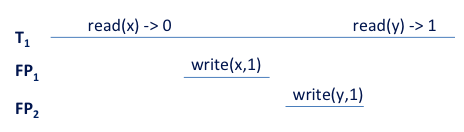
\includegraphics[width=\columnwidth]{figs/FP-semantics}
\caption{Possible violation of real-time order among fast path transactions. Regular transaction $T_1$
reads $x$ before it is updated by fast path transaction $FP_1$ and reads $y$ after it is updated by fast path transaction $FP_2$ even 
though $FP_2$ occurs after $FP_1$. 
%$T1$'s global version is $10$, and its skips the local version clocks of the regions holding $x$ and $y$ to $10$ when reading from them.
}
\label{fig:ltx-rt}
\end{figure}
} % remove
Specifically, %our correctness condition stipulates that
the system enforces a total order ${\cal T}$ on all committed transactions, so that
\begin{enumerate}
    \setlength{\itemsep}{0pt}
    \setlength{\parskip}{0pt}
    \setlength{\parsep}{2pt}  
%\item
%regular transactions (though not FP ones) are ordered in ${\cal T}$  according to their commit times;
\item
non-overlapping transactions 
%(regular and FP) 
that update the same key occur in ${\cal T}$  in order of their commit times;
\item
each  transaction's read operations see a consistent snapshot of the database reflecting 
a prefix of  ${\cal T}$; 
%and  
%that includes at least all regular transactions committed prior to its start time; and 
\item
 a transaction commits only if none of the items it updates is modified by a transaction ordered in ${\cal T}$ after
 its snapshot time and before its commit time.
 \end{enumerate}

\remove{ % OLD SI definition - no relaxation of RTO
More precisely, 
SI enforces a total order on committed transactions according to their commit times so that 
\begin{enumerate}
    \setlength{\itemsep}{0pt}
    \setlength{\parskip}{0pt}
    \setlength{\parsep}{2pt}  
\item
each transaction's read operations see a consistent snapshot of the database reflecting write operations by
 exactly those transactions that committed prior to the transaction's start time; and 
\item
 a transaction commits only if none of the items it updates has been modified since that snapshot.
 \end{enumerate}
 } %Remove
 
Note that as with SI, two concurrent transactions conflict only if they both \emph{update} the same item.  
In contrast, under serializability, a transaction that updates an item also conflicts with transactions that \emph{read} that item. 
Snapshot isolation is thus amenable to implementations (using multi-versioning) that 
allow more concurrency than serializable ones, and hence scale better.
It is provided by popular database technologies such as Oracle, PostgreSQL, and SQL Server,
and TPSs such as Percolator, Omid, and  CockroachDB.

Following a commit call, the transaction may successfully \emph{commit}, whereby all of its operations take effect, 
or 
%in case of conflicts, (i.e., when two concurrent transactions attempt to update the same item), the transaction may
\emph{abort}, in which case none of its changes take effect. 



%An abort may also be initiated by the programmer, e.g., 
%on encountering an error. Applications typically retry a transaction upon  abort. 


%%%The data is \emph{partitioned} (or sharded), and each object belongs to one region. 
%%%%Global transactions may span multiple regions, and atomically commit or abort on all. 
%%%\emph{Local transactions} are ones that access a single region.



\subsection{TPS operation schema}
\label{ssec:schema}

\begin{figure}
\centerline{
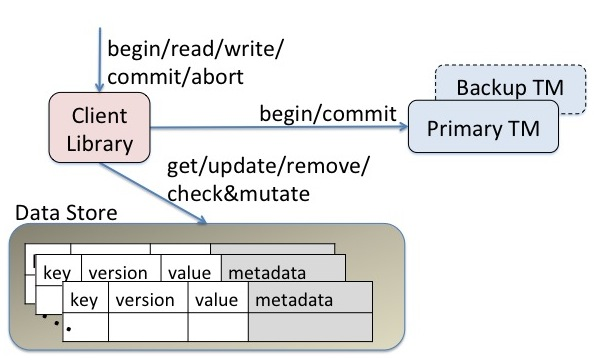
\includegraphics[width=0.45\textwidth]{FragolaComponents.jpg}
}
\caption{Transaction processing architecture: A client library exposes an  API for  executing transactions of data store operations. 
A centralized Transaction Manager (TM) handles transaction begin and commit requests, while data is written directly to the 
underlying data store. The TM has a backup for high availability.}
\label{fig:components}
\end{figure}

Figure~\ref{fig:components} depicts, at a high level, the primary components of the TPS architecture,  
their API's, and interaction with the data store. 

In many TPSs, transaction processing follows the following general schema, 
outlined in Algorithm~\ref{alg:schema}, while systems vary in their implementations of each of the steps.

\remove{
For example, whereas most systems rely on a centralized service for timestamp allocation~\cite{OmidICDE2014,Omid2017,tephra,Percolator2010}, this is not essential~\cite{cockroach}; similarly, validation (conflict detection) can use a centralized service~\cite{OmidICDE2014,Omid2017,tephra}, per-transaction entries in a global table~\cite{cockroach}, or distributed locking and validation~\cite{Percolator2010}. 
Different ways to implement this schema are  discussed in Section~\ref{sec:context}.
We now overview the phases a transaction goes through, focusing on Omid's approach.
}

\begin{algorithm}[tb]
\begin{algorithmic}[1]
%\small
\Procedure{begin}{}
\State obtain read timestamp $ts_r$ 
\EndProcedure
%\Statex

\Procedure{write}{$ts_r$, key, value} \Comment transactional write
\State optionally check for conflicts and abort if found 
\State indicate write intent for key with value and $ts_r$
\State add key to local write-set
\EndProcedure
%\Statex

\Procedure{read}{$ts_r$, key} \Comment transactional read
\If{key has write intent}
	\State resolve, possibly abort writing transaction \label{l:resolve}
\EndIf
\State return highest version   $\le ts_r$ of key
\EndProcedure

%\Statex

\Procedure{commit}{$ts_r$, write-set}
\Statex \Comment check for write-write conflicts  \label{l:validate}
\State obtain commit timestamp $ts_c$
\If{validate(write-set, $ts_r$)}  
%	\Statex \Comment commit all write intents with version $ts_c$
	\State write commit  version $ts_c$ to persistent commit entry \label{l:commit}
\Else
	\State abort	
\EndIf
\State post-commit: update meta-data
\EndProcedure

\end{algorithmic}
\caption{TPS operation schema.} 
\label{alg:schema}
\end{algorithm} 

Most of the systems employ a centralized \emph{transaction manager (TM)\/} service~\cite{Percolator2010,OmidICDE2014,Omid2017,tephra},
 sometimes called timestamp oracle, for timestamp allocation and other functionalities. 
 Because a centralized service can become a single point of failure, the TM is sometimes implemented
 as a primary-backup server pair to ensure its continued availability following failures.

\mypara{Begin.} 
  When a transaction begins, it obtains a read timestamp (version) $ts_r$ for reading its consistent snapshot.
  %, and unique transaction id.   The two can be combined (i.e., $ts_r$ can serve as the  transaction id, provided that it is unique).
 In most cases, this is done using the centralized TM~\cite{Percolator2010,OmidICDE2014,Omid2017,tephra}. 
%  In CockroachDB, the timestamp is based on a local clock that is ``close to'' real-time and preserves causality 
 % across regions, and unique transaction ids are used to break ties in case timestamps (from different regions) are identical. 

\mypara{Transactional writes.} 
 During a transaction, a write operation indicates its \emph{intent} to write to a single object a certain new value with a certain version number.
%a dedicated \emph{commit} column in the object indicates that the write is tentative.
In Omid, the version is the transaction's $ts_r$, which exceeds all versions written by transactions that committed before the
current transaction began. Note that the version order among concurrent transactions that  attempt to update the same key is immaterial, 
since all but one of these transactions are doomed to abort. 

It is possible to buffer write intents locally (at the client) in the course of the transaction, and add the write intents to the data store at commit time~\cite{Percolator2010}.

In some solutions writes check for conflicts before declaring their intents~\cite{cockroach}, whereas in others, 
all conflict detection is deferred to commit time~\cite{Percolator2010,OmidICDE2014,Omid2017,tephra}. 

\mypara{Transactional reads.} 
The reads of a given transaction obtain a consistent snapshot of the data store at logical time (i.e., version) $ts_r$.
Each read operation retrieves the value of a single object associated with the highest timestamp that is 
smaller or equal to the transaction's $ts_r$. 

On encountering a write intent, read cannot proceed without determining whether the tentative write should be included in its snapshot,
for which it must know the writing transaction's commit status. 
To this end, TPSs keep per-transaction \emph{commit entries}, which are the source of truth regarding the transaction status 
(pending, committed, or aborted). 
This entry is updated in line~\ref{l:commit} of Algorithm~\ref{alg:schema} as we explain below, 
and is checked in order to resolve write intents in line~\ref{l:resolve}.
In some cases~\cite{Percolator2010,cockroach}, when the status of the writing transaction  is undetermined, the read forcefully aborts
it by updating the commit entry accordingly, as explained below.

%Similarly, the solution we implement in \sys\ forces the transaction with the pending write intent to abort. 

  \mypara{Commit.} 
  Commit occurs in four steps:
  \begin{enumerate}
    \setlength{\itemsep}{0pt}
    \setlength{\parskip}{0pt}
    \setlength{\parsep}{2pt}  
  \item
  Obtain a commit timestamp, $ts_c$. 
  In most cases, e.g.,~\cite{Percolator2010,OmidICDE2014,Omid2017,tephra}, 
  this is the value of some global clock maintained by a centralized entity. 
  \item \emph{Validate} that the transaction does not conflict with any concurrent transaction that has committed since it 
had begun.  For SI, we need to check for write-write conflicts only. 
If write intent indications are buffered, they are added at this point~\cite{Percolator2010}.
Validation can be centralized~\cite{OmidICDE2014,Omid2017,tephra} or distributed~\cite{Percolator2010,cockroach}. 


\item \emph{Commit} or abort in one  irrevocable atomic step by persistently writing to the \emph{commit entry}, 
  which can reside in a global table~\cite{Omid2017,cockroach} or alongside the first  key written by 
  the transaction~\cite{Percolator2010}.  
  
 \item \emph{Post-commit}: 
  Finally, a transaction changes its write intents to
  persistent writes in case of commit, and removes them in case of abort. This
  step is not essential for correctness, but reduces the overhead of future transactions. It
  occurs after the transaction is persistently committed or aborted via the commit entry, 
  and can be done asynchronously.
  %in
  %order to reduce the overhead of future transactions (by sparing them the need to check the commit entry)
  %and to garbage collect   obsolete information. 
 \end{enumerate}
 
  \remove{Note that whenever a transaction encounters a write
  indication in the collect phase it must access the commit entry in order to
  check the transaction's commit status. Once the post-commit phase is over, future
  transactions no longer incur this overhead for keys updated by the terminated
  transaction.}

\subsection{Big data platforms}
\label{ssec:bigdata}

{\inred{

Apache HBase is one of the most scalable key-value storage technologies available today. 
Like many state-of-the-art data stores, it scales through horizontal \emph{sharding} 
(partitioning) of data across \emph{regions}. An HBase instance is deployed 
on multiple nodes (\emph{region servers}), each of which typically serves hundreds 
of regions. Production HBase clusters of 1K nodes and above are becoming common. 
For example, Yahoo Japan leverages an HBase cluster of $3{,}800$ nodes 
that collectively store $37$PB of data~\cite{yahoojapanhbase}. 

Phoenix complements the HBase storage tier with a query processing (compute)
tier. The latter scales independently (the current scalability goal is $10{,}000$ query servers). 
Phoenix compiles every SQL statement into a plan, and executes it on one or more servers. 
Its query processing code invokes the underlying HBase for low-level data access, and a 
TPS (Omid or Tephra) for transaction management, through client libraries. 

Wherever possible, Phoenix strives to push computation close to data (e.g., for filtering
and aggregation), in order to minimize cross-tier communication. For this, it makes 
extensive use of server-side stored procedures, which in HBase are supported by the 
non-intrusive {\em coprocessor\/} mechanism. Omid uses HBase coprocessors too, either for 
performance improvements or for specific services (e.g., garbage collection of redundant 
data). 
}}